\documentclass[11pt, oneside]{article}   	% use "amsart" instead of "article" for AMSLaTeX format
\usepackage{geometry}                		% See geometry.pdf to learn the layout options. There are lots.
\geometry{letterpaper}                   		% ... or a4paper or a5paper or ... 
%\geometry{landscape}                		% Activate for rotated page geometry
%\usepackage[parfill]{parskip}    		% Activate to begin paragraphs with an empty line rather than an indent
\usepackage{graphicx}				% Use pdf, png, jpg, or eps§ with pdflatex; use eps in DVI mode
								% TeX will automatically convert eps --> pdf in pdflatex		
\usepackage{amssymb}

\usepackage{graphicx}
\graphicspath{ {img/} }

%SetFonts

%SetFonts


\title{Testing LSD-SLAM using synthetical images}
\author{Zili Wang}
%\date{}							% Activate to display a given date or no date

\begin{document}
\maketitle
%\section{}
%\subsection{}
\section{Introduction}
I generate some simple scenes and objects in Unity3d, and walk in the scene and render it into images sequences. Then feed these images into LSD SLAM. I find it comes in great handy if I want to test the feature of a algorithm. Just by causally adjusting the setting of the scene, I find that:\\
1, The width of view is very important in tracking.\\
2, If you want to get the dense points of a object, you should make the object cover the major area of the rendered image. Otherwise, it is very easy to lose tracking.\\

\section{Result}
\subsection{Test tracking in open scene}
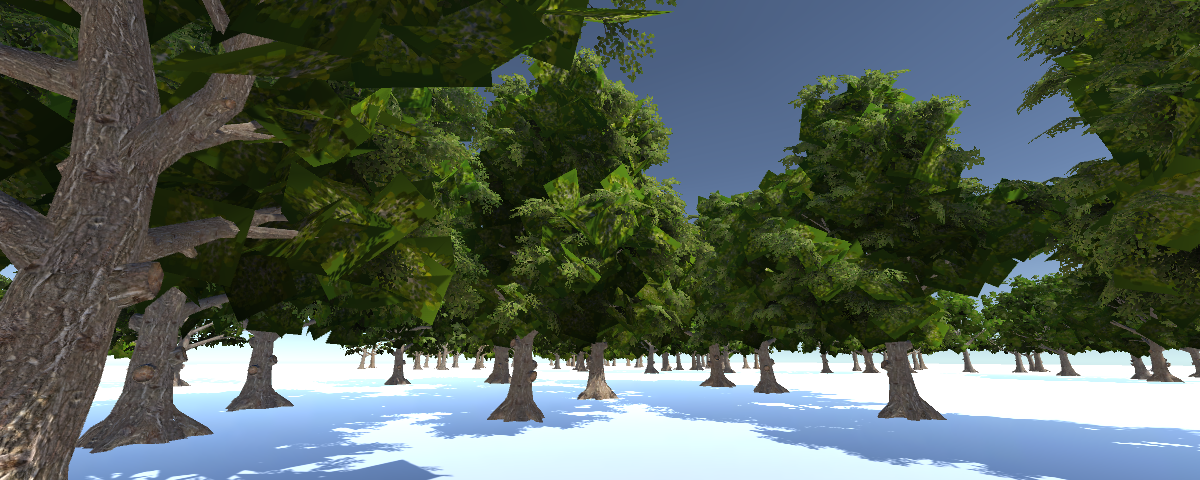
\includegraphics[width=1.0\textwidth]{i4}\\
One frame of the open scene\\
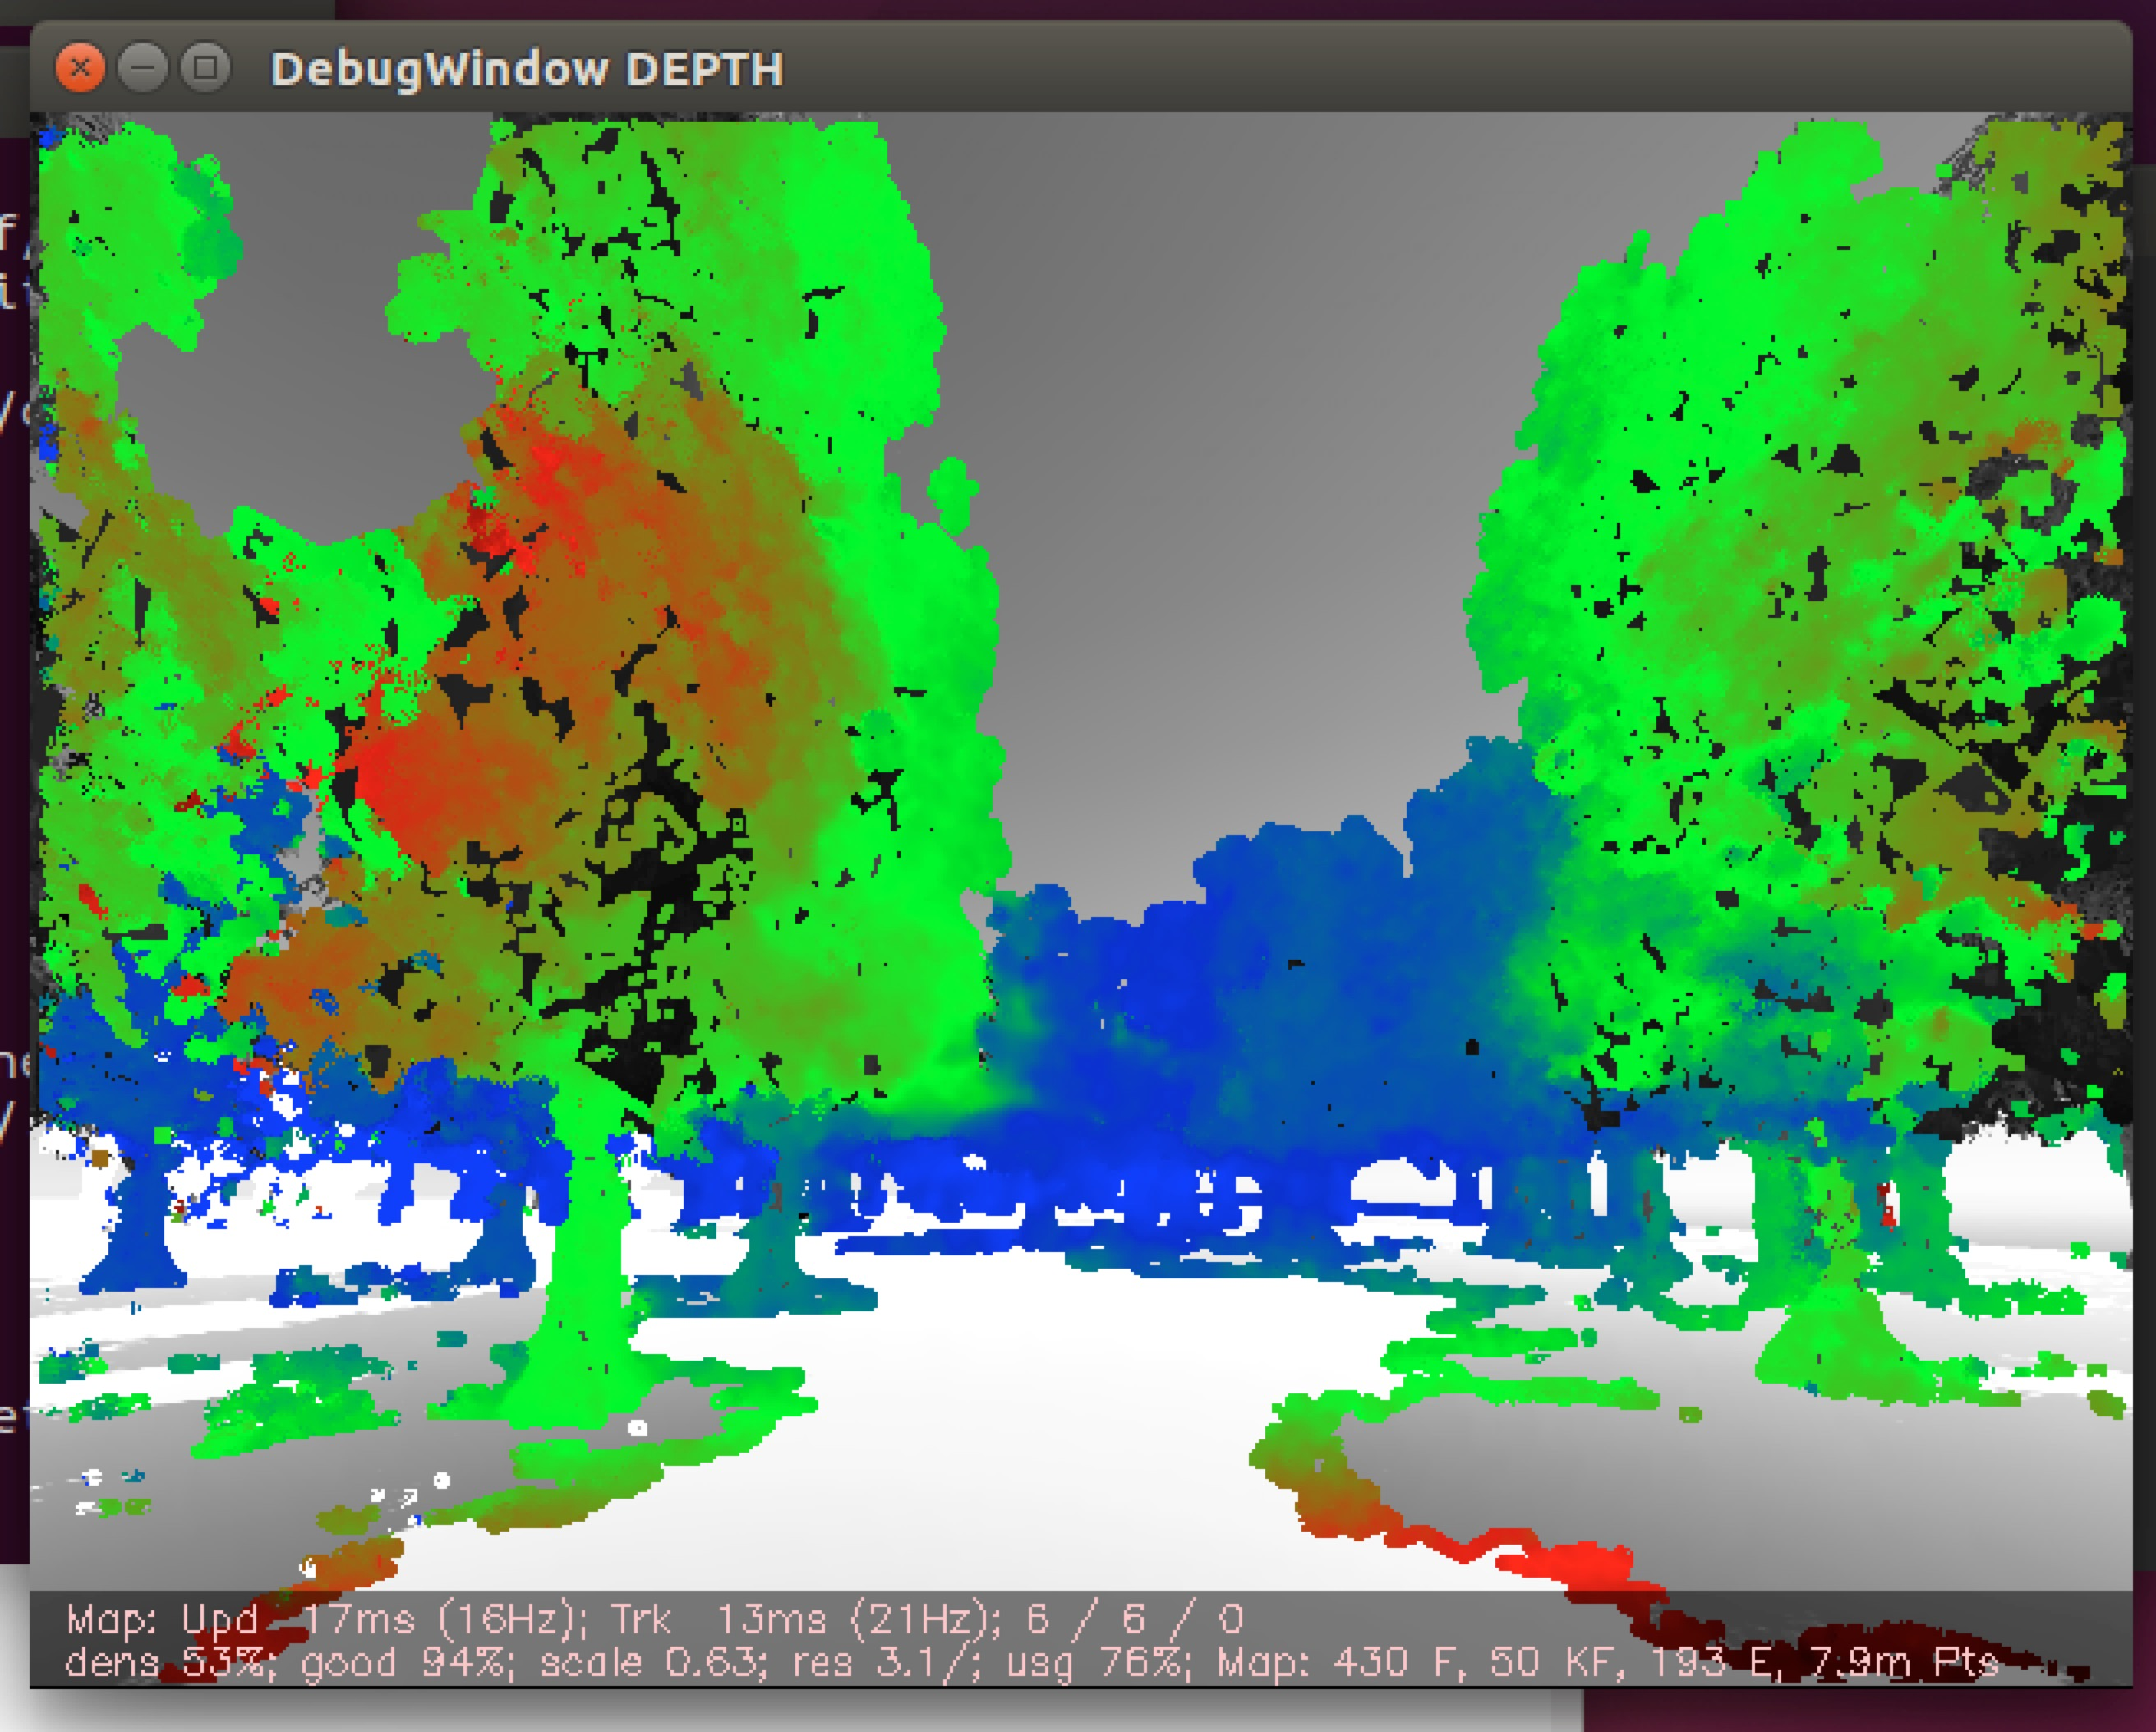
\includegraphics[width=0.8\textwidth]{i3}\\
One frame of the open scene with dense point overlapped\\
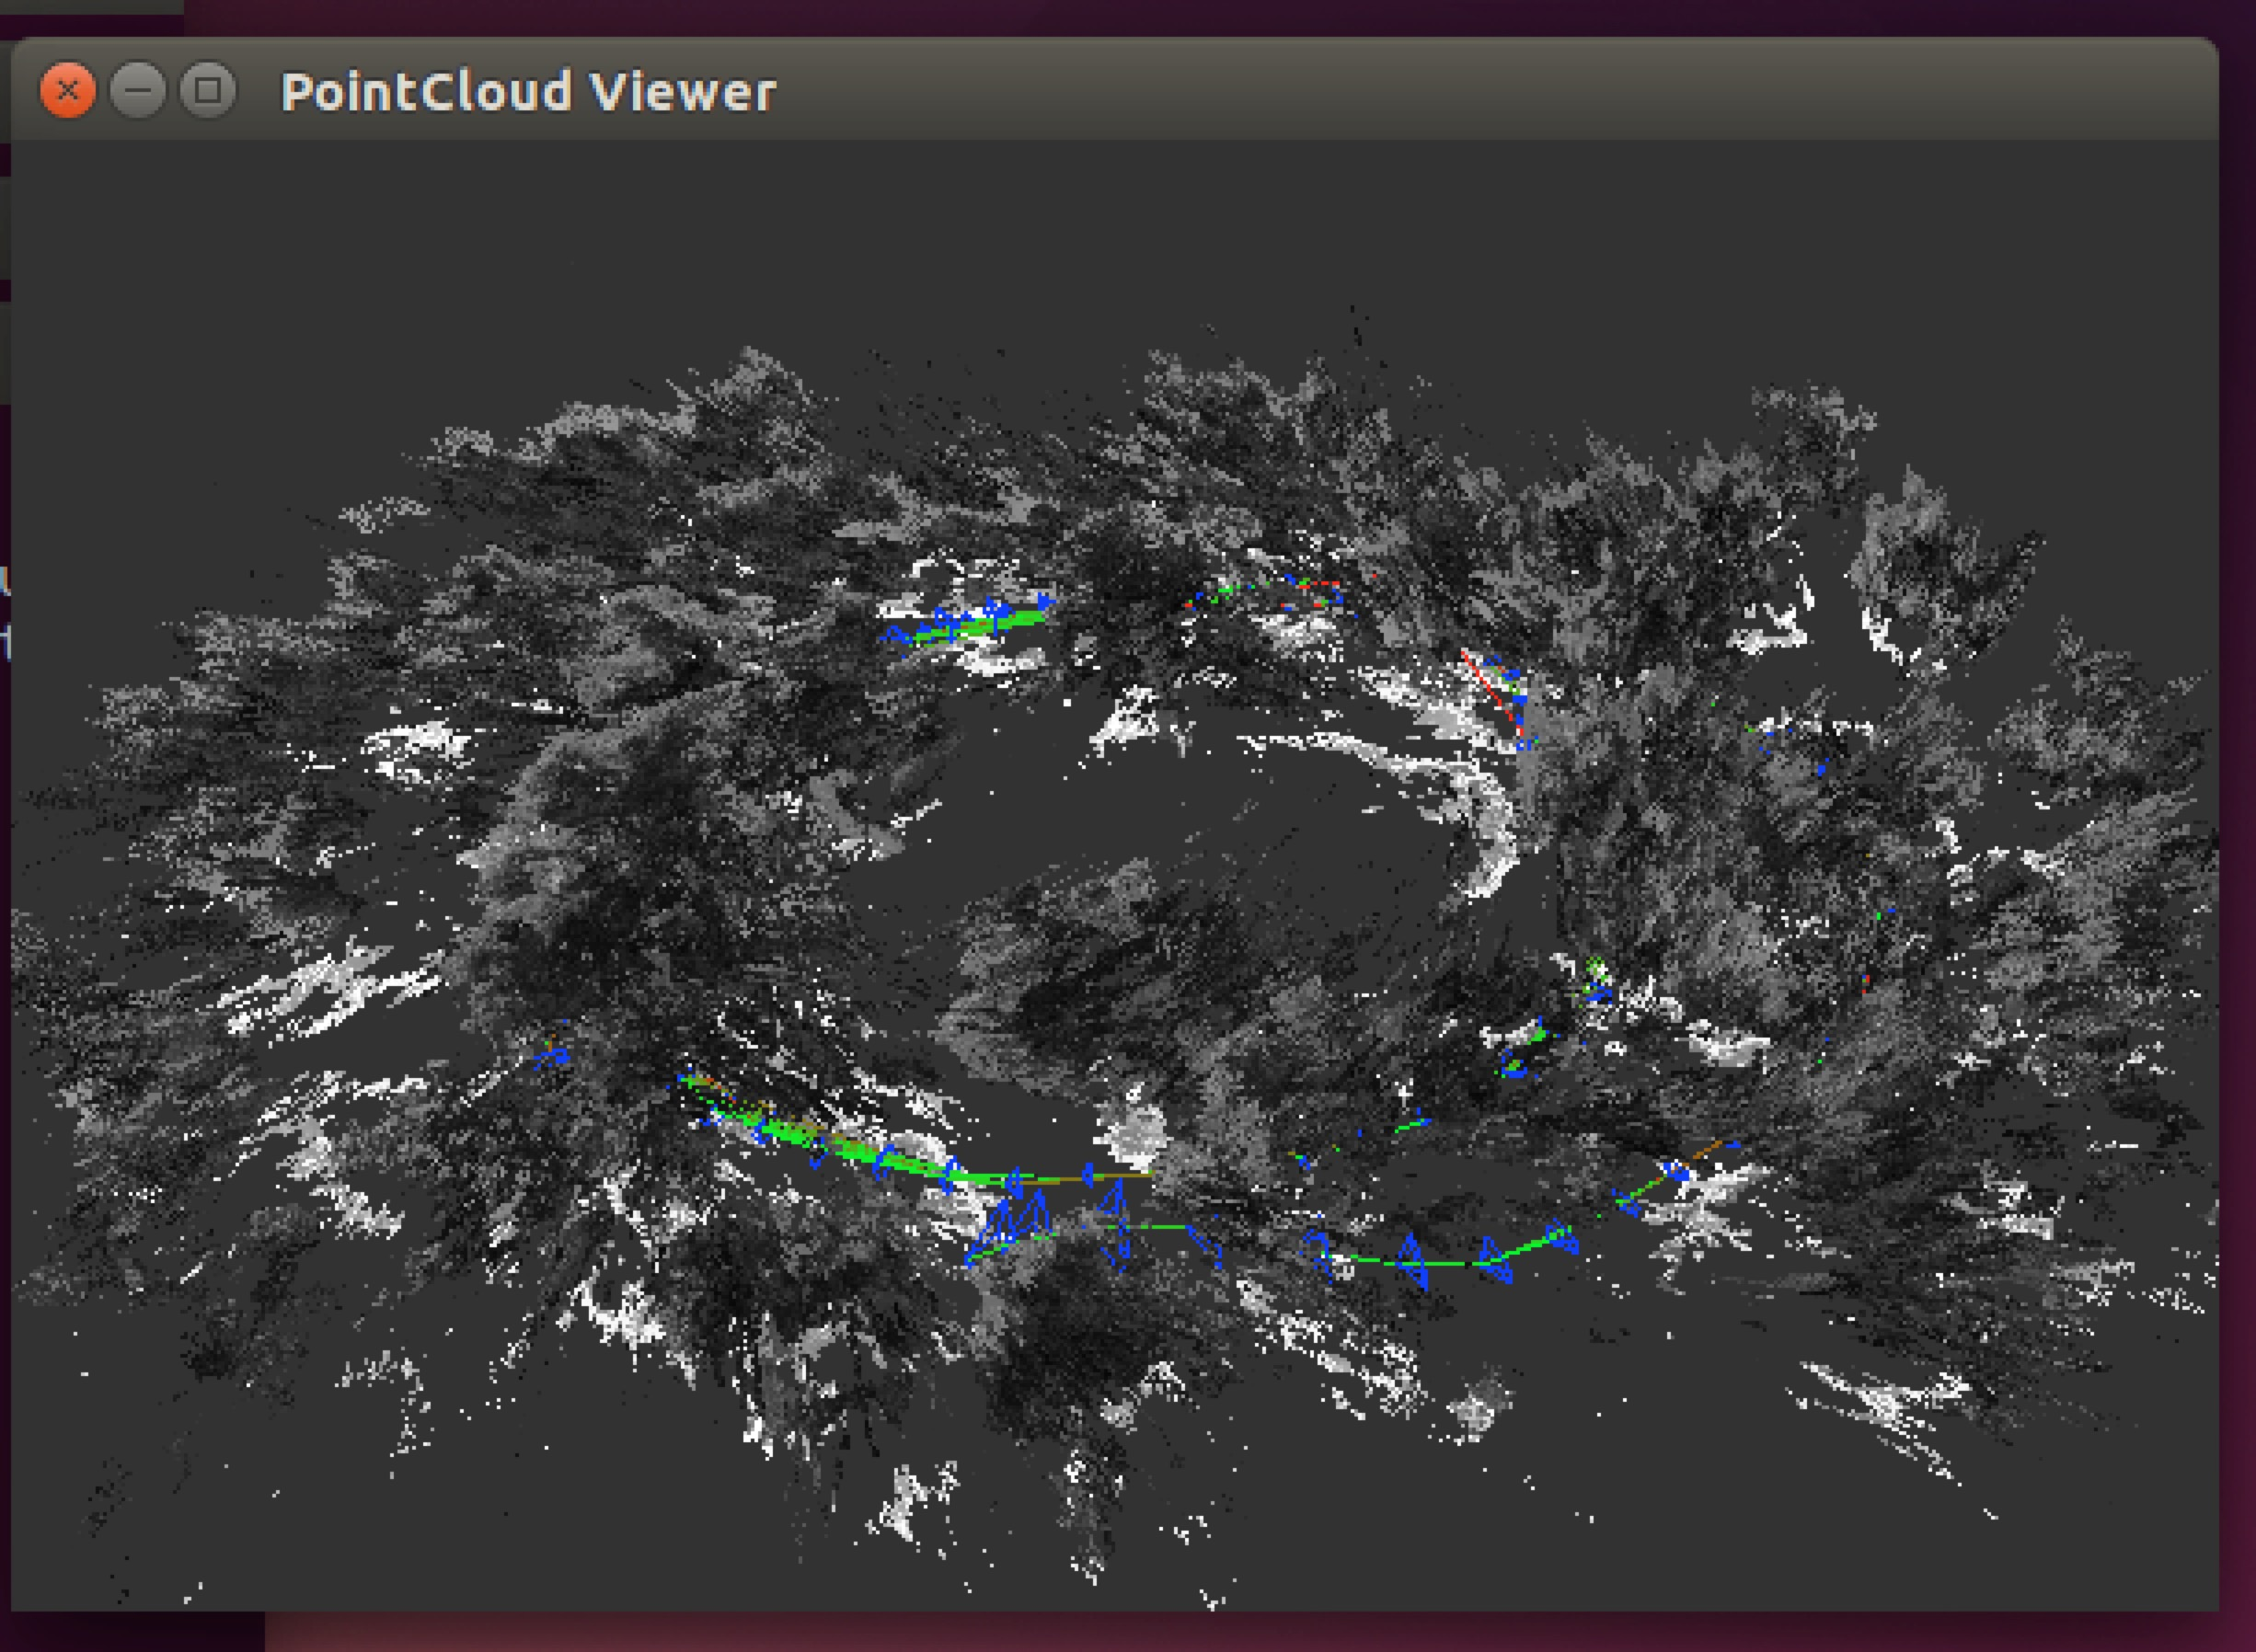
\includegraphics[width=0.8\textwidth]{i1}\\
Trajectory with dense points\\
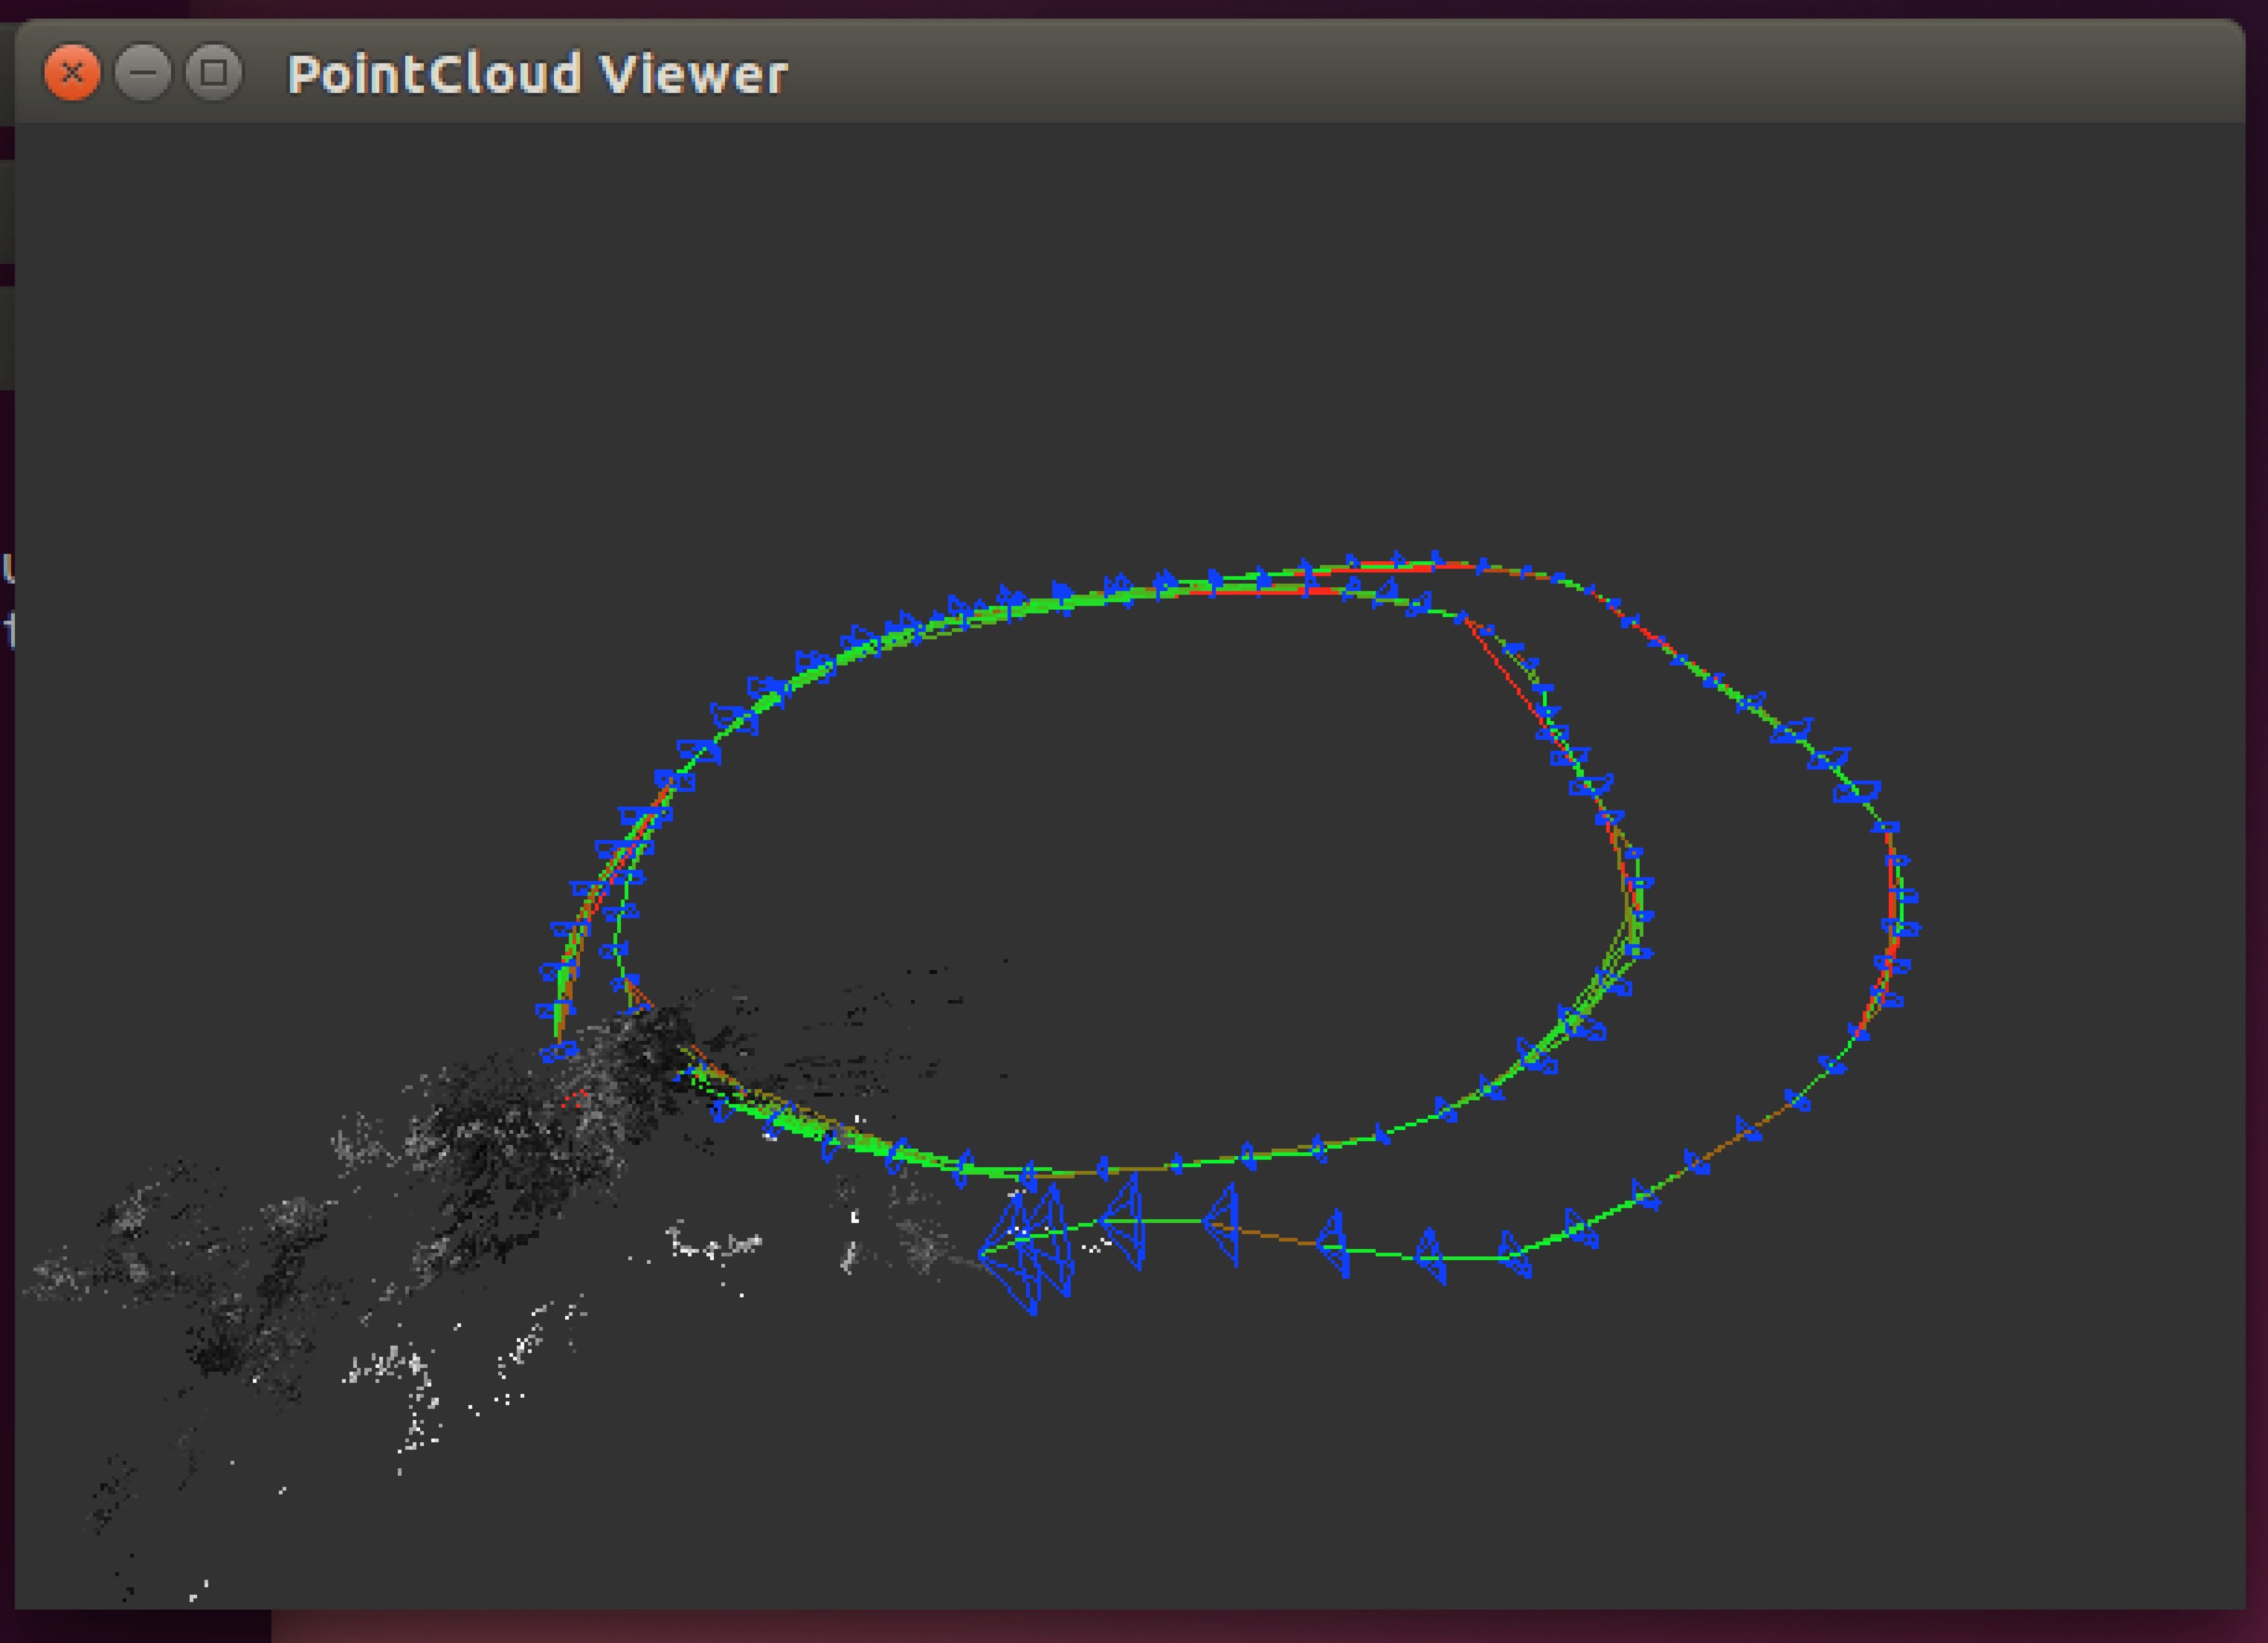
\includegraphics[width=0.8\textwidth]{i2}\\
Trajectory \\

\subsection{Test mapping by a object}

\includegraphics[width=1.0\textwidth]{i5}\\
One frame of the object\\
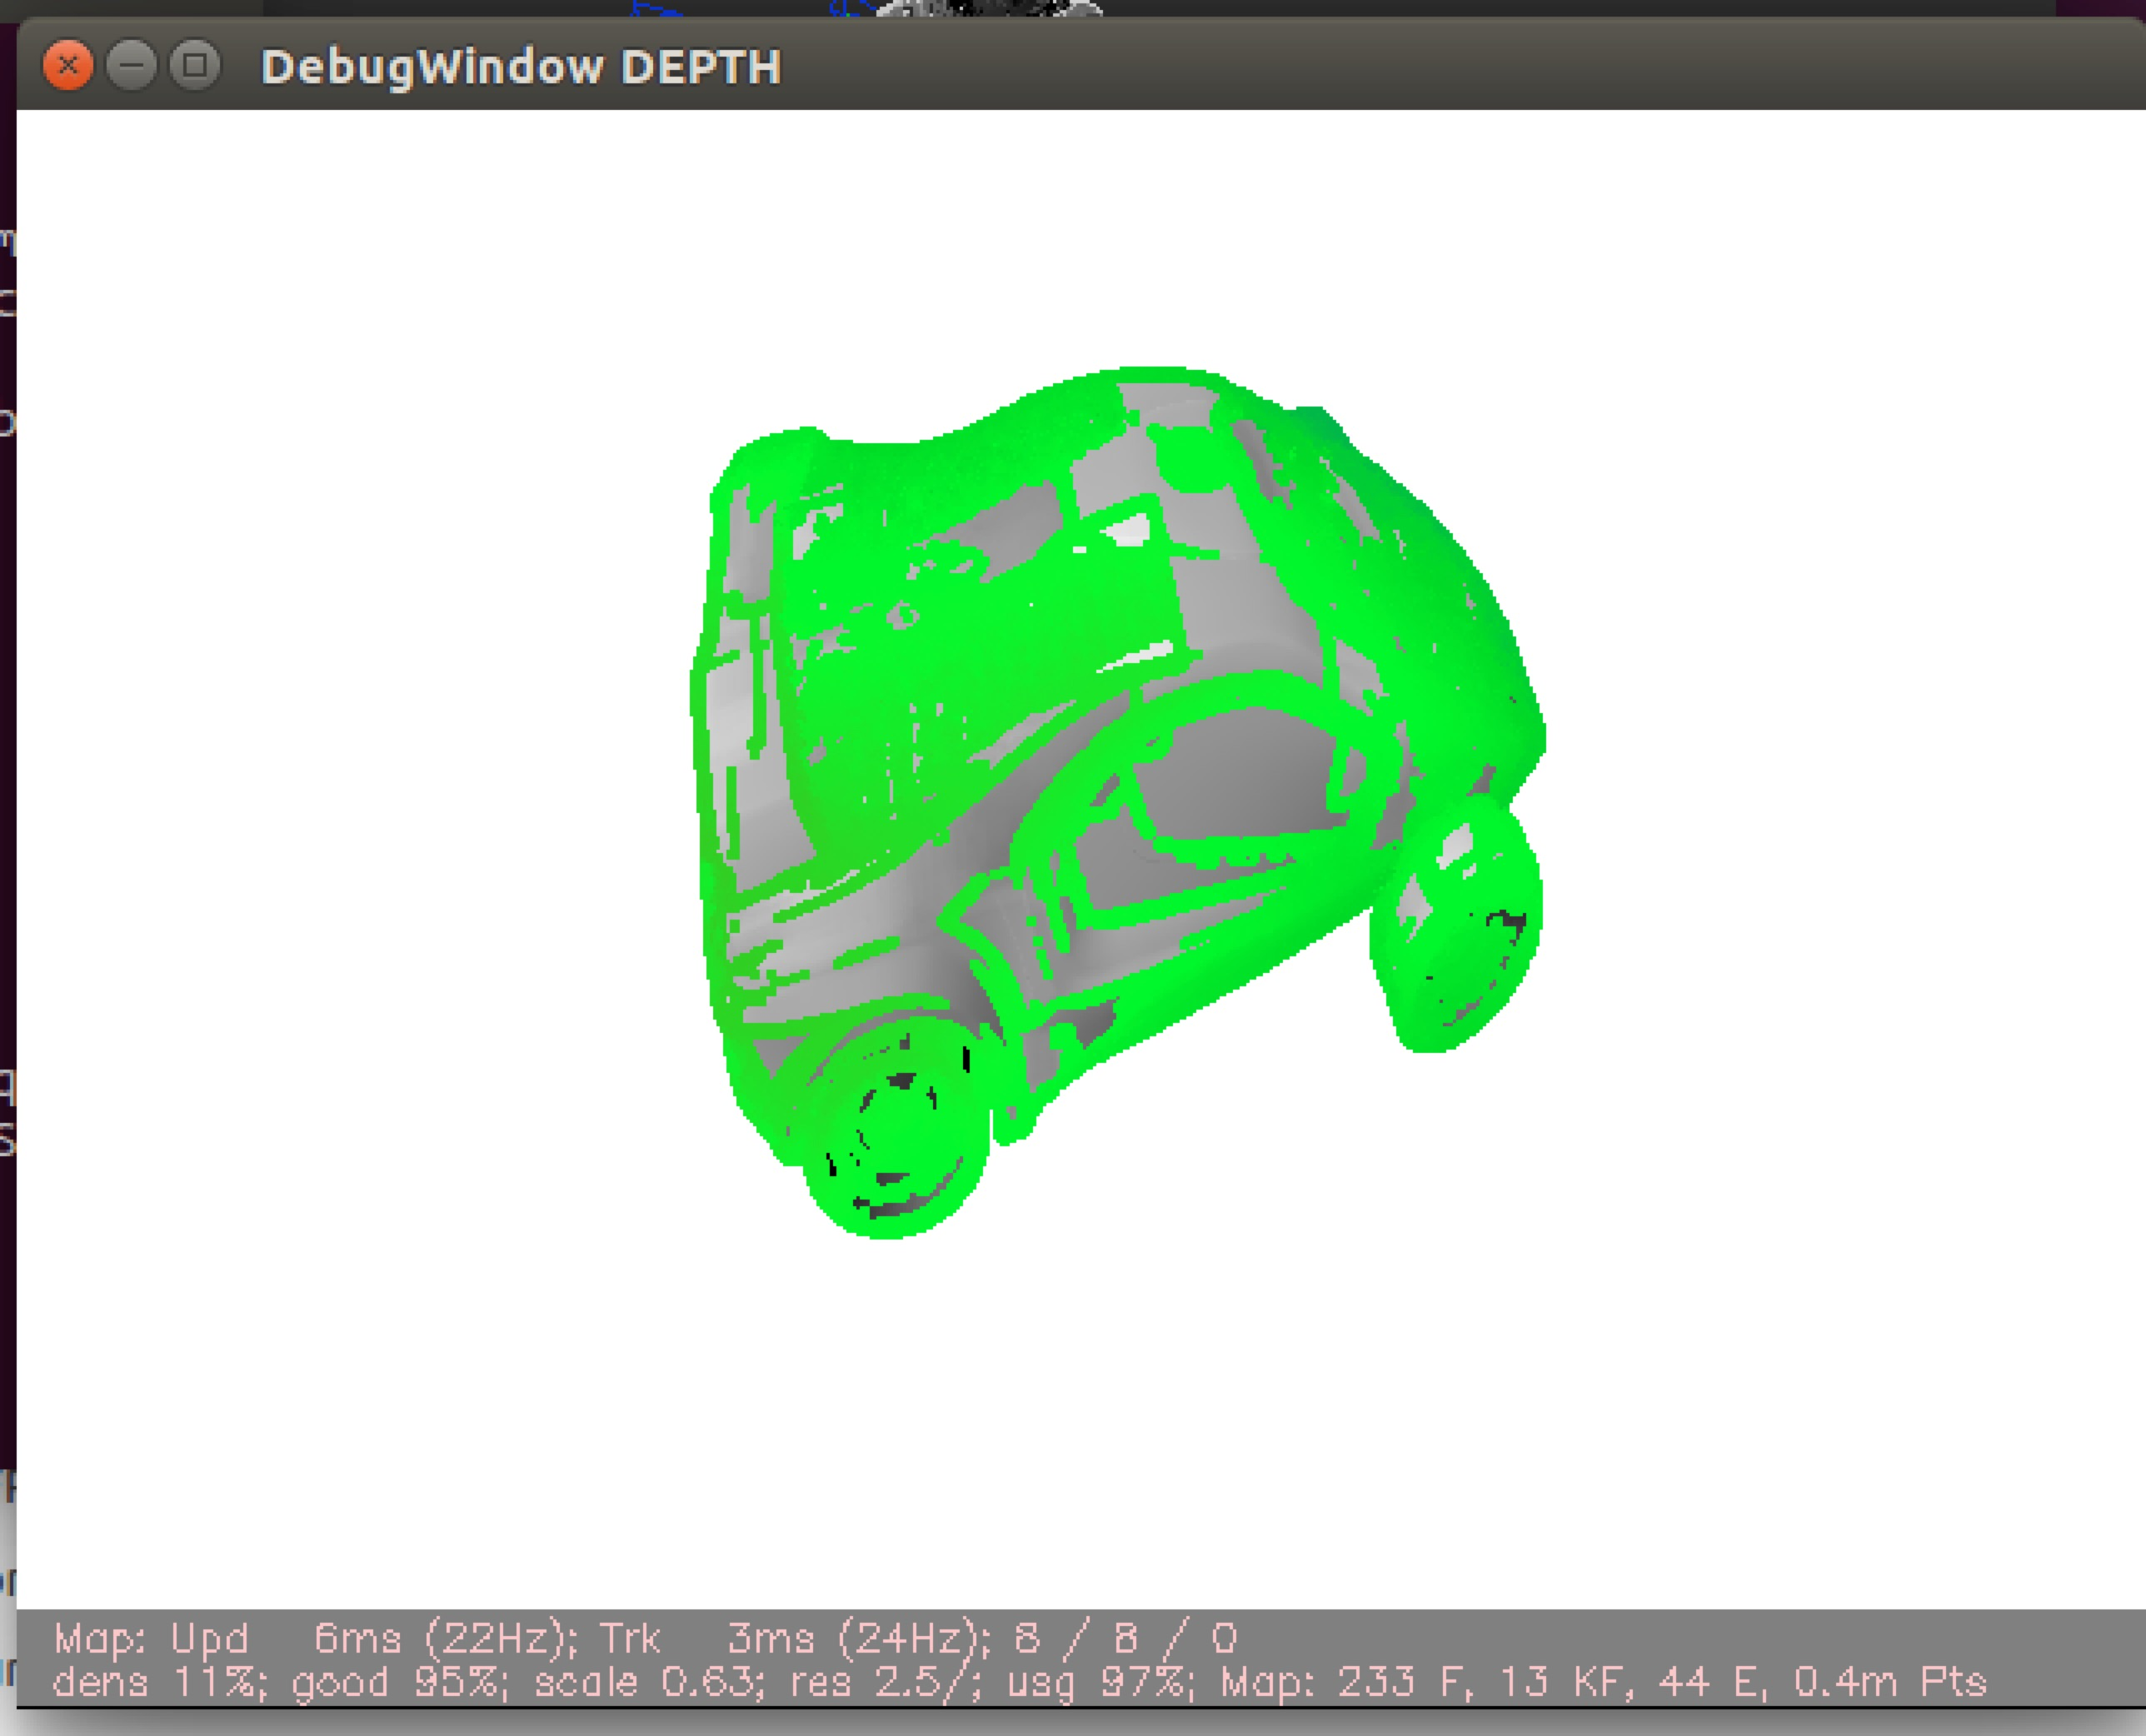
\includegraphics[width=0.8\textwidth]{i9}\\
One frame of the object with dense point overlapped\\
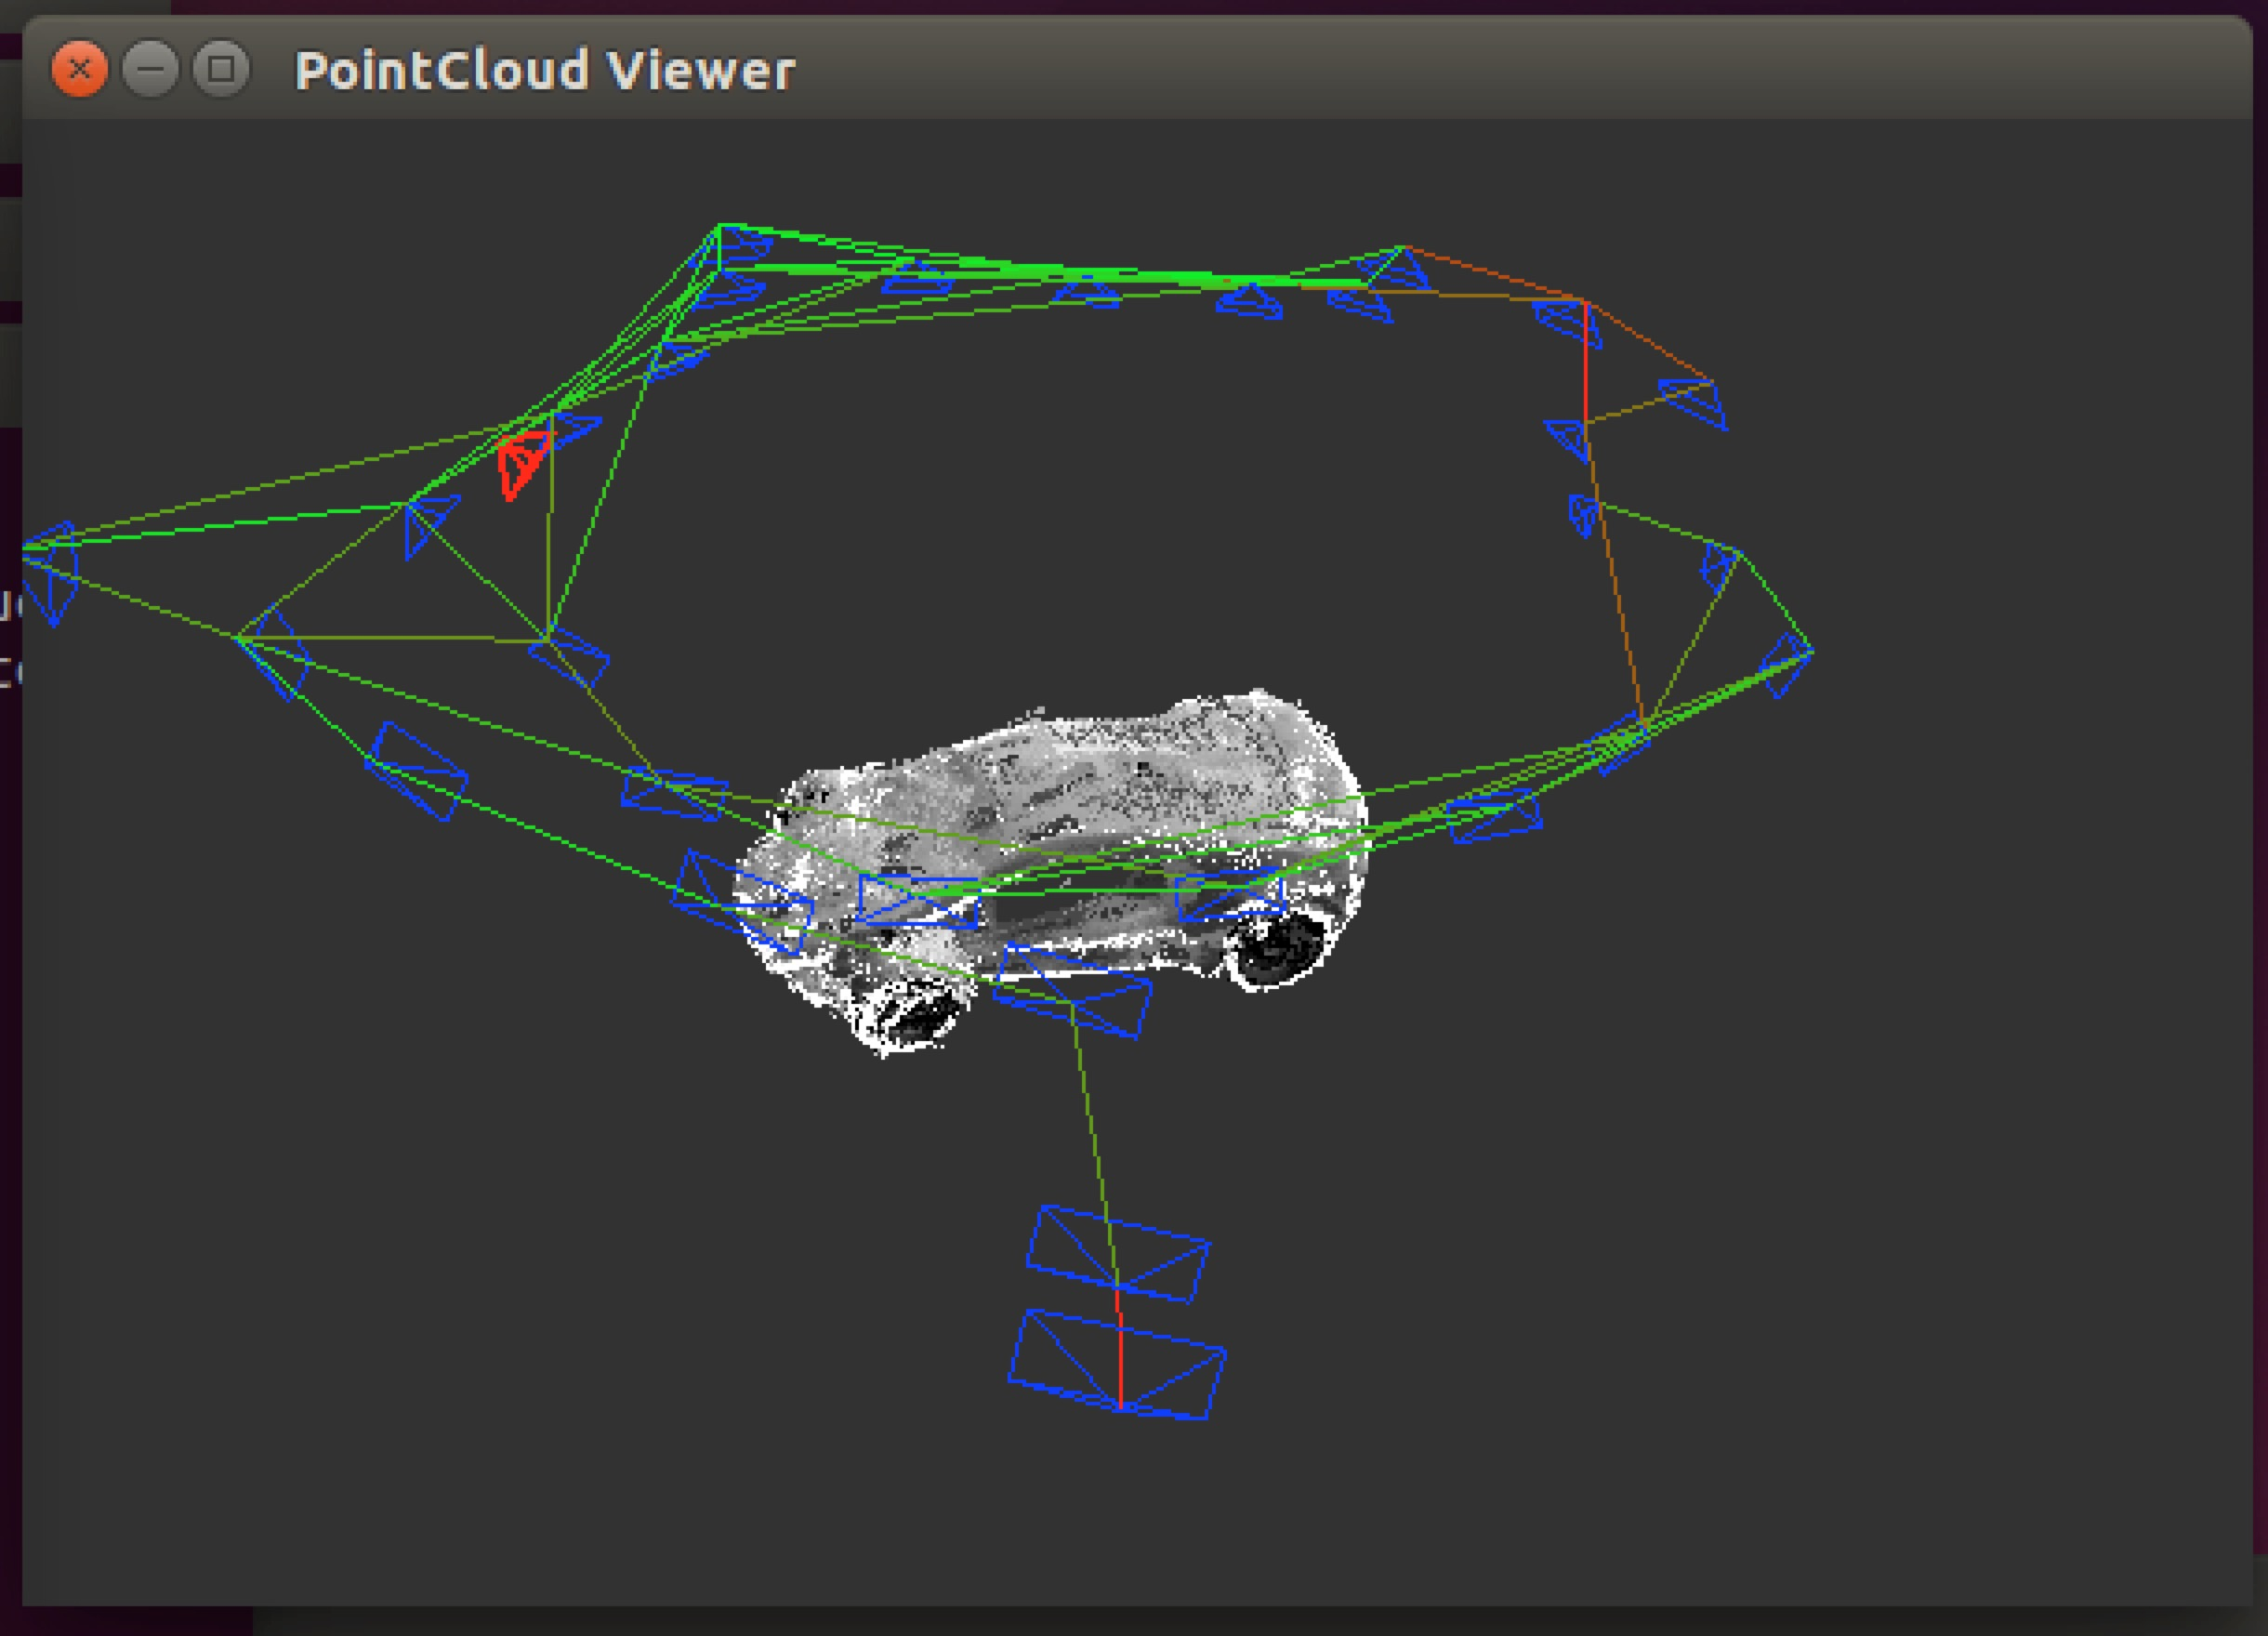
\includegraphics[width=0.8\textwidth]{i6}\\
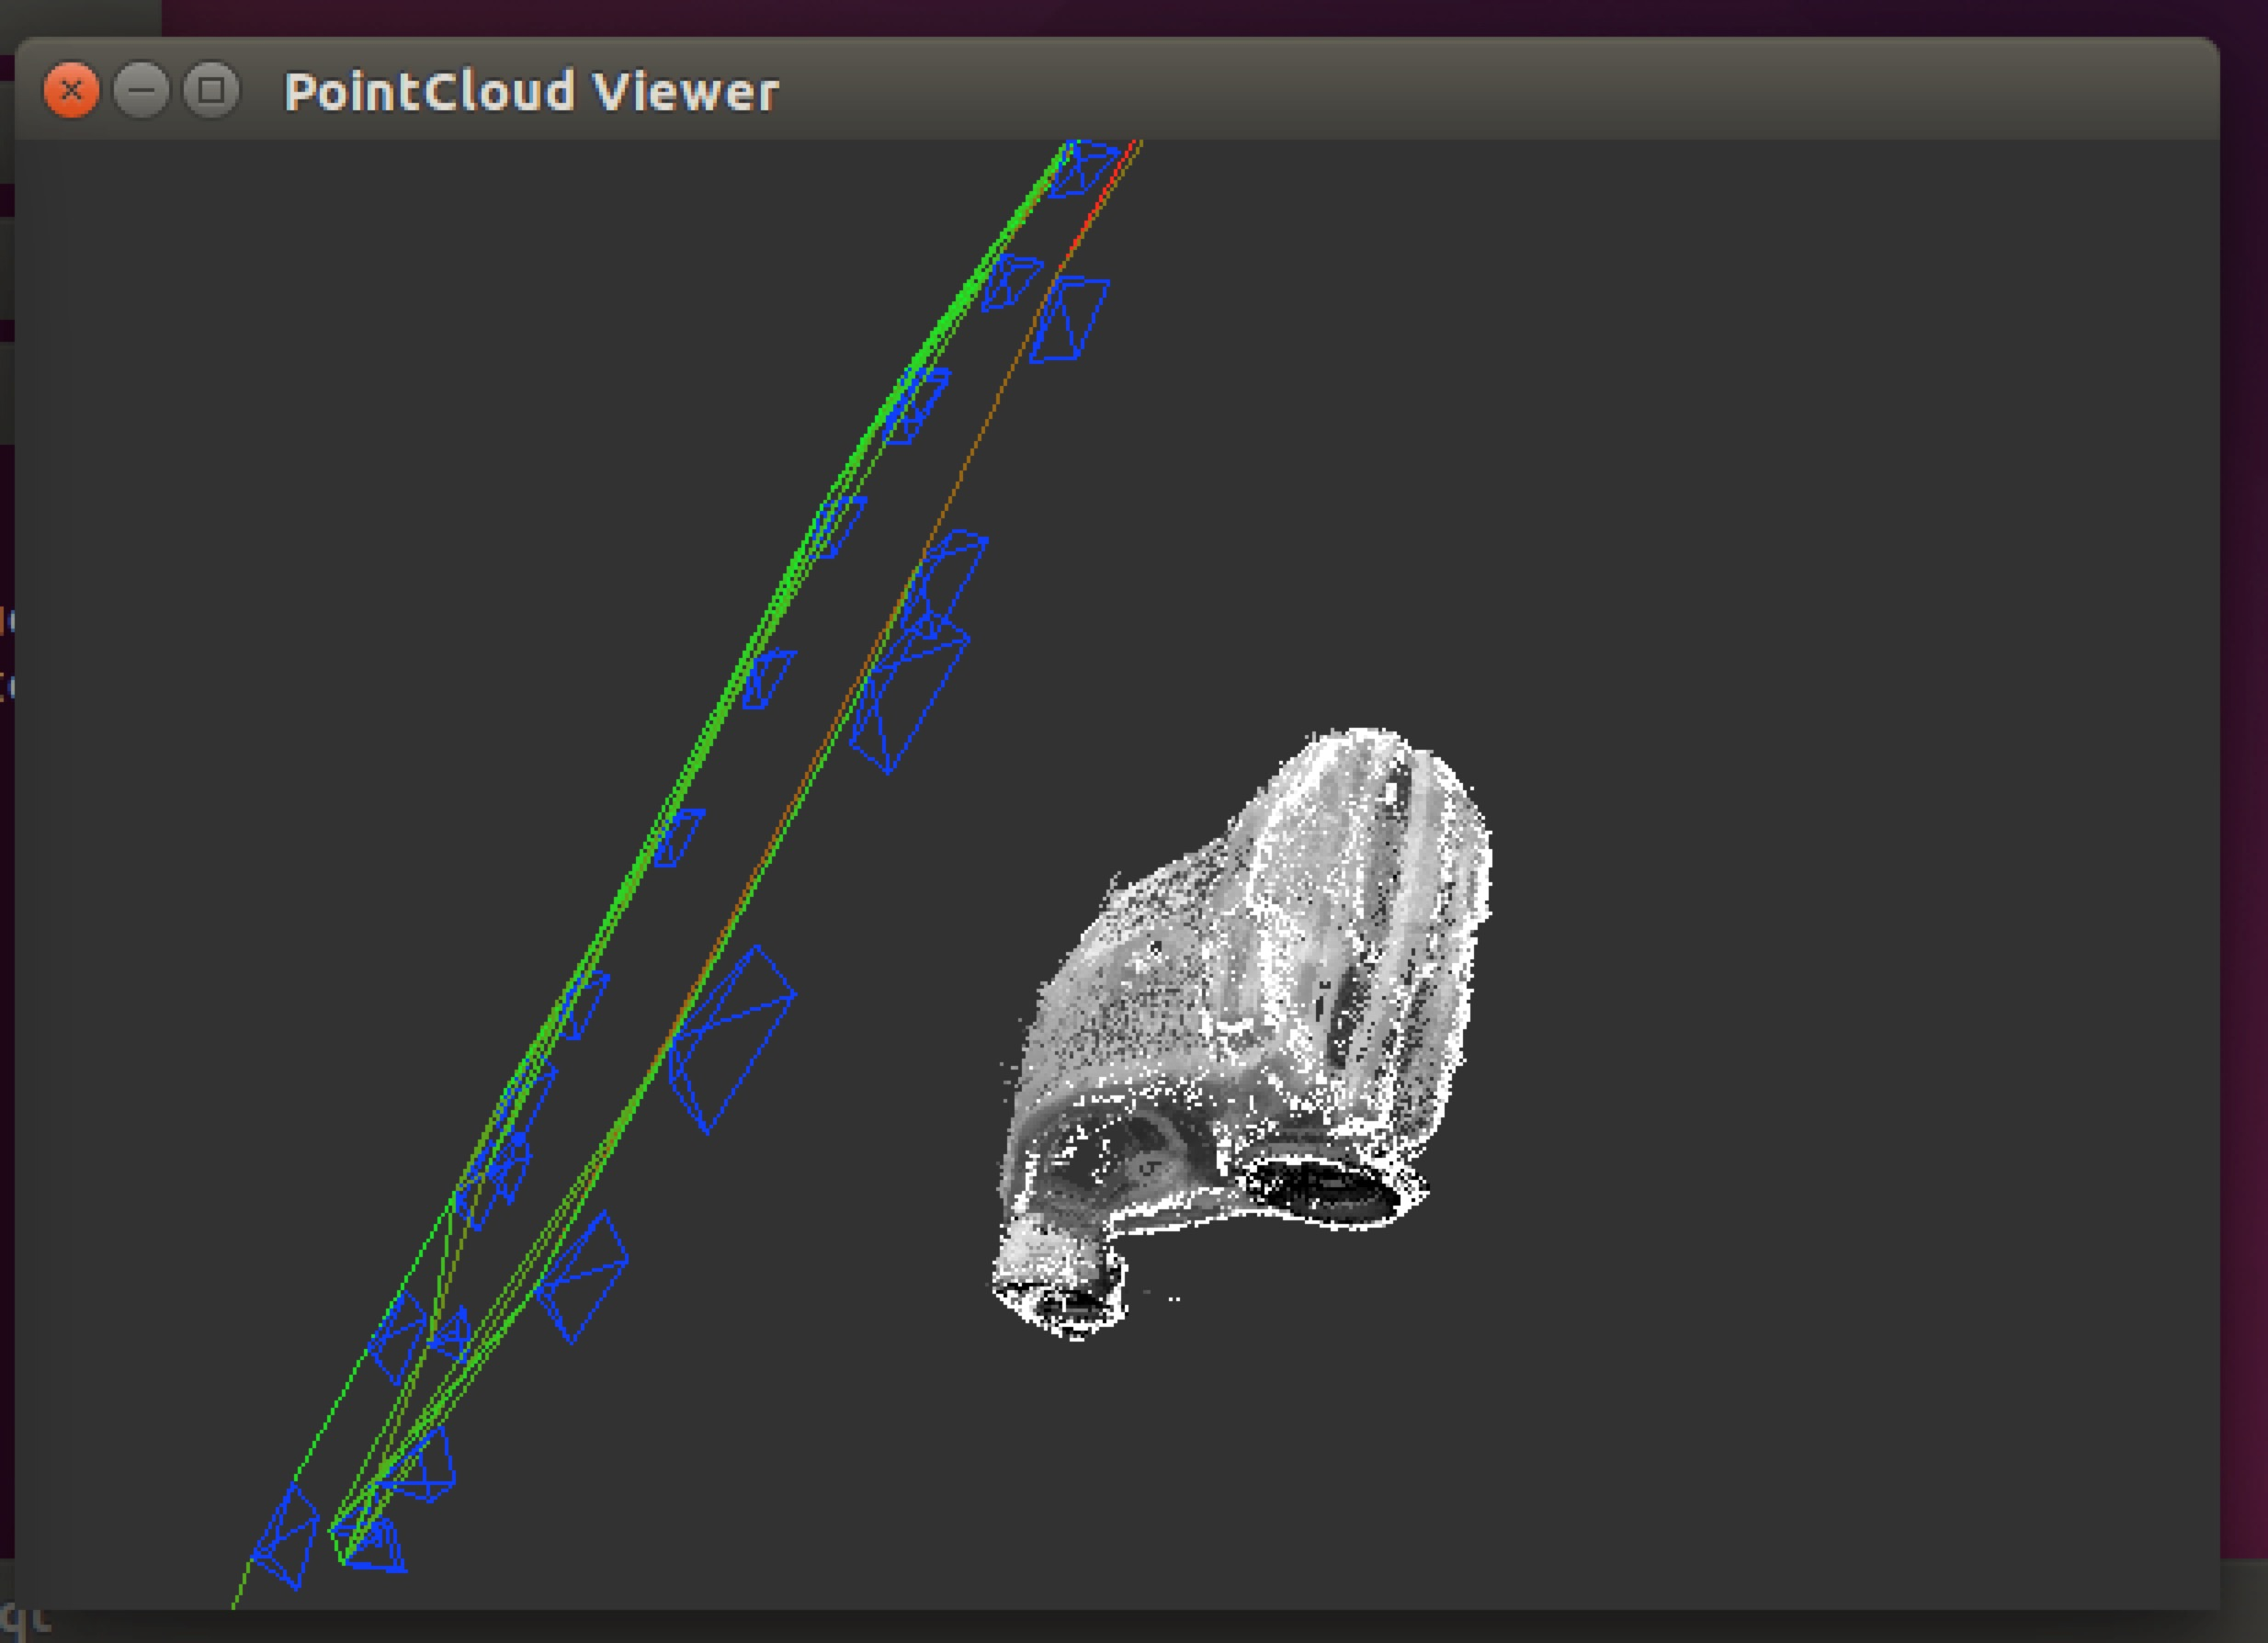
\includegraphics[width=0.8\textwidth]{i7}\\
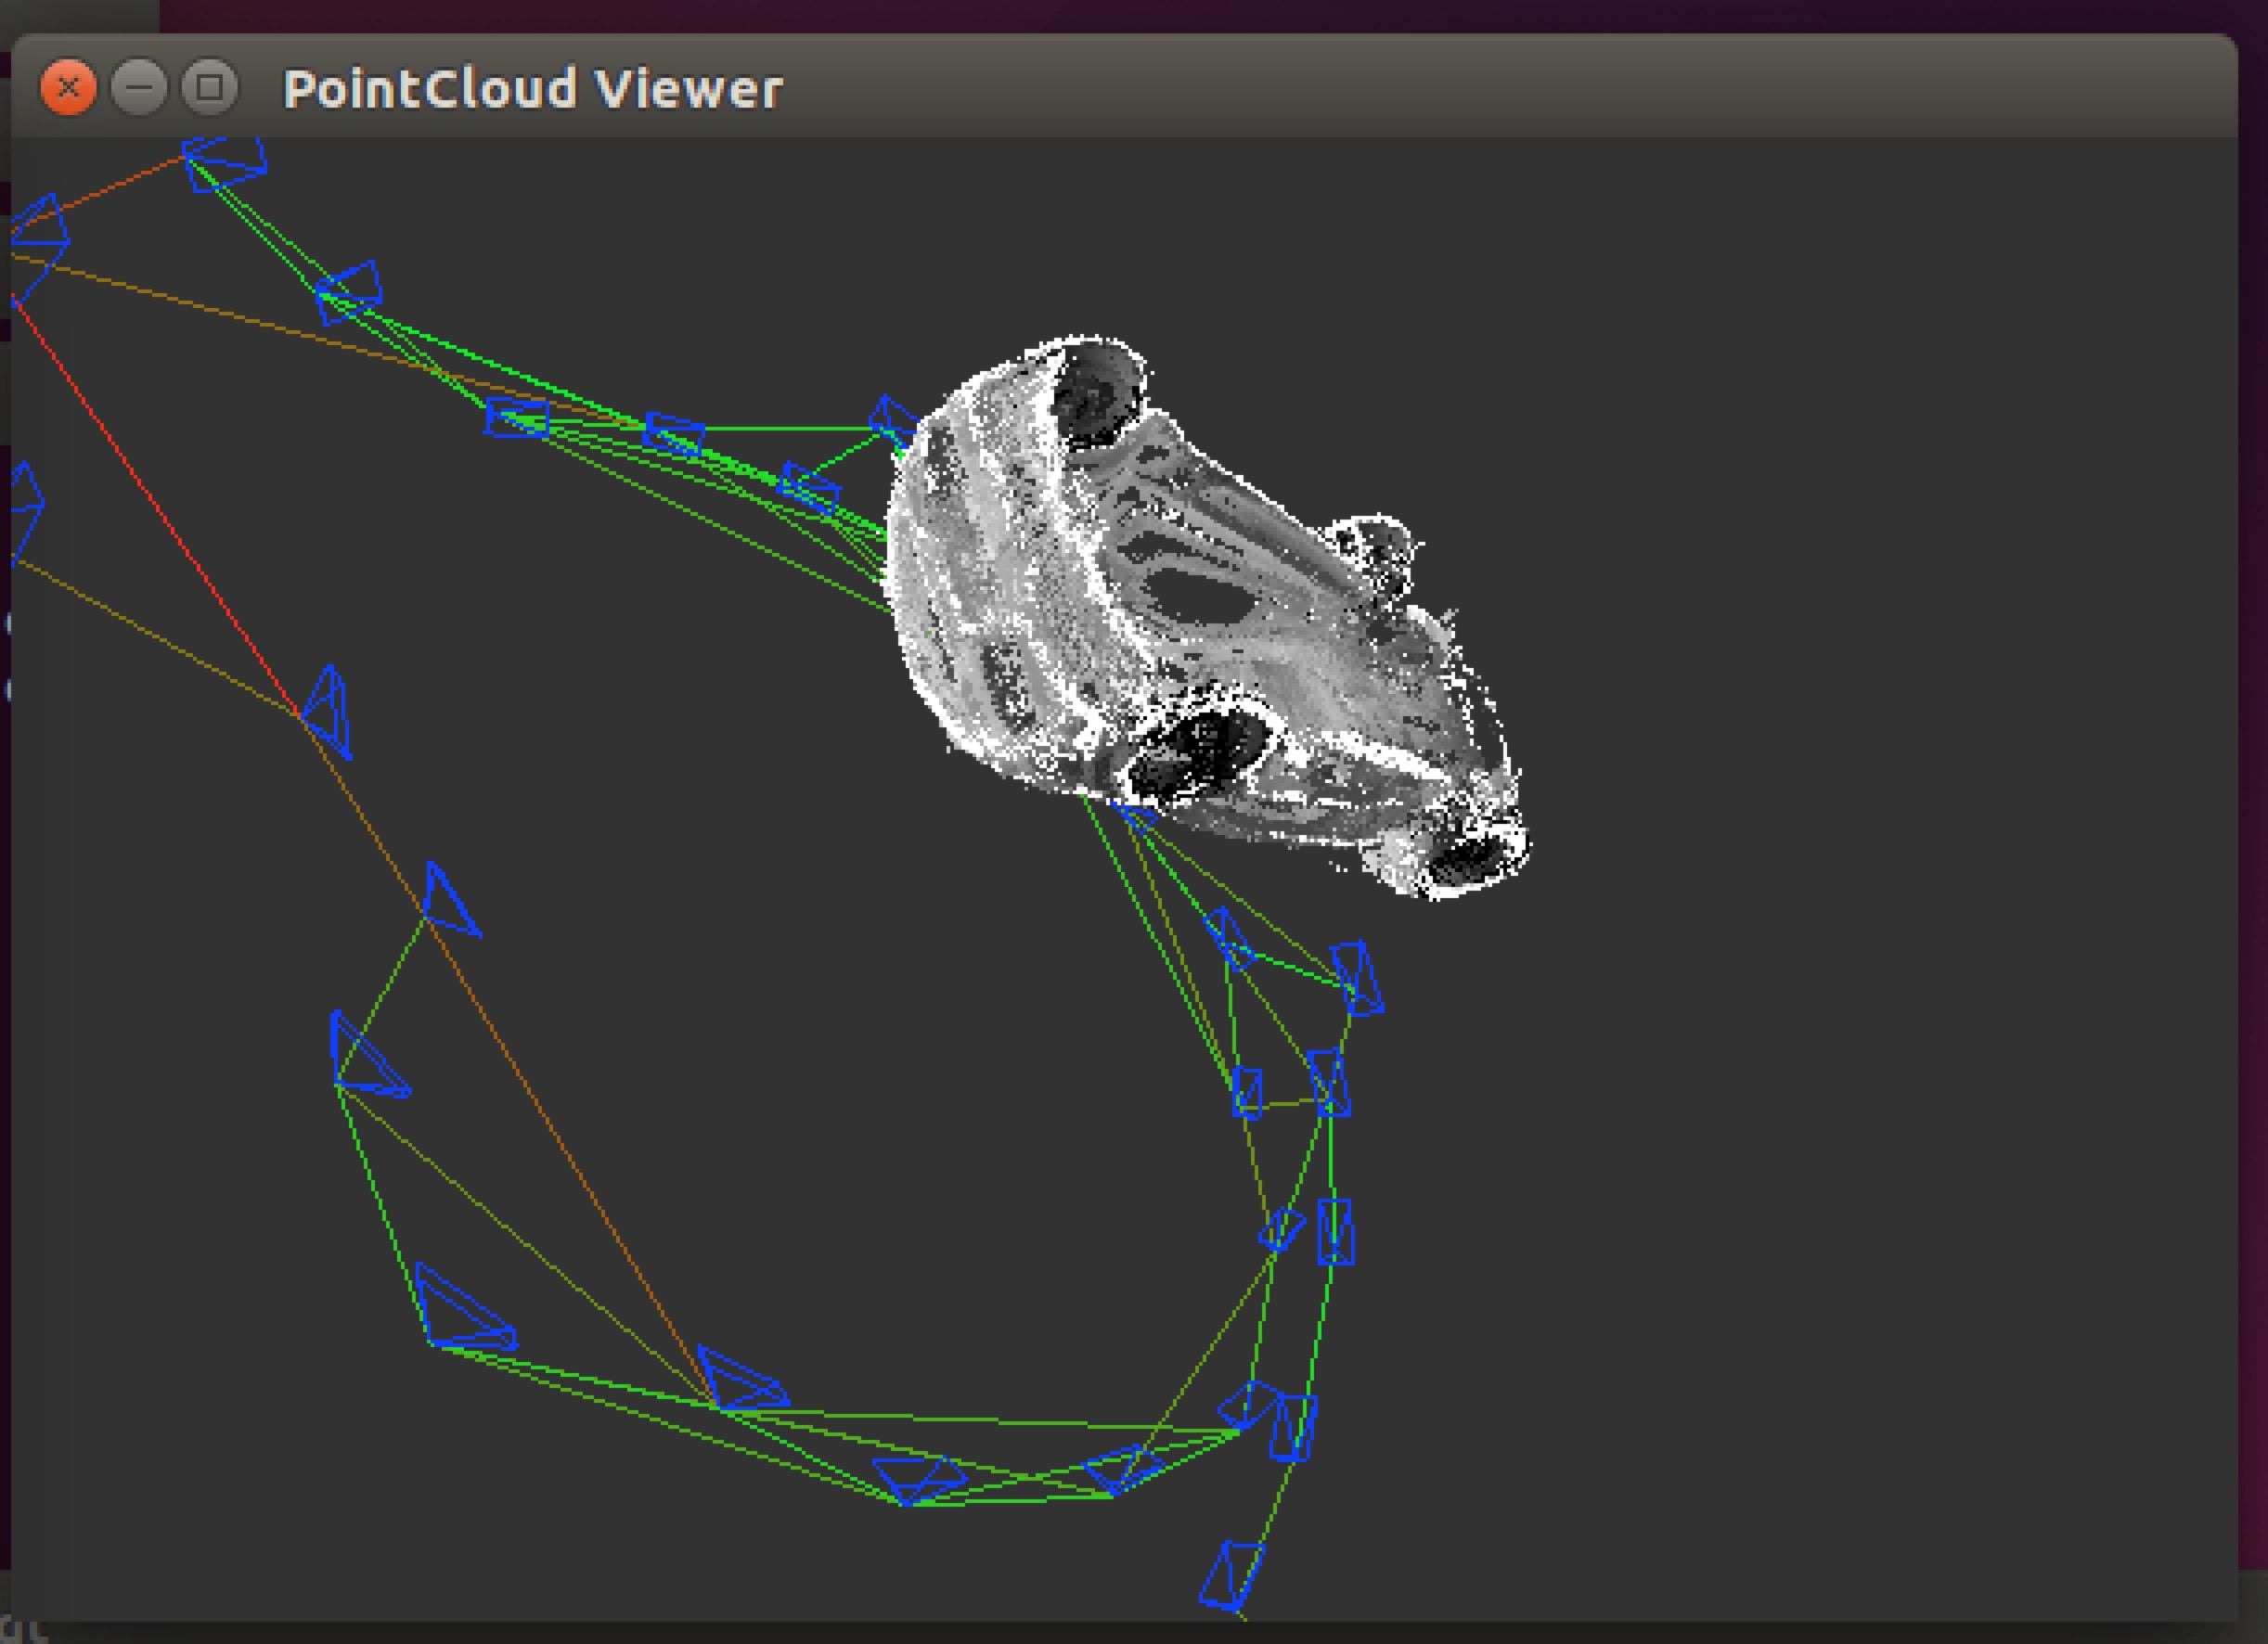
\includegraphics[width=0.8\textwidth]{i8}\\
Trajectory with dense model\\

\end{document}  